\section{Experimental Results}
\label{Experimental Results}

We used the simulator to examine the results of the game between the adversary and the utility described in \ref{Game}.  We examined the effectiveness of our four proposed adversarial strategies and our suggested defense techniques under two different scenarios.  In the first, there are an equal number of each class of customer.  In the second, 40\% are Bakeries, 40\% are Batteries, and 20\% are Buckets.  All of our results are over 15,000 total customers in order to make our distribution assumptions accurate.  Further, the results presented here are average over 10 different random number seeds in order to eliminate any bias in a given sample from the distributions.

\begin{figure}[!htbp]
\centering
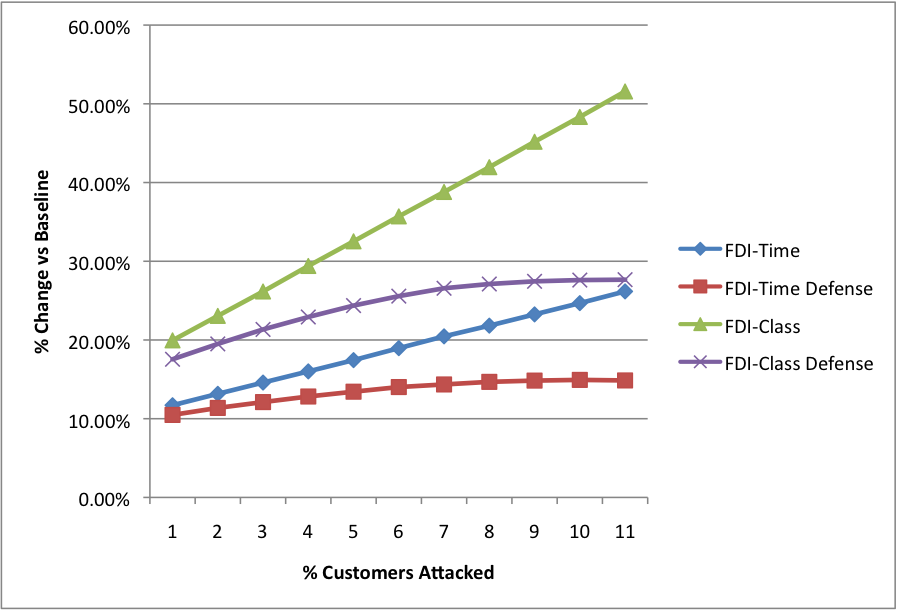
\includegraphics[width=.5\textwidth]{equal-attacks.png}
\caption{Attack strategies with equal numbers of customers in each class}
\label{equal-attack}
\end{figure}

Figure \ref{equal-attack} shows the results for the first scenario, with 5,000 Bakeries, Batteries, and Buckets.  The first important thing to note is that in all cases the defense strategy halves the efficacy of the attack.  It is also interesting ot compare the efficacy of the different classes of attack.  Both the jamming attack and the false data injection - load attack are essentially ineffective.  Both permute the load of a subset of bakeries by ~20\%, which is not enough to have a significant effect of the utility's scheduling problem, and shows the efficacy of existing techniques for dealing with this problem.  However, the time and class injections had a large impact, at 26\% and 52\% respectively.  Both of these attacks are only made possible by the advent of the smart grid and the addtional information that it communicates.  Our defensive investment strategy was able to decrease the malicious effects to 14\% and 27\% respectively.  This illustrates that these new vulnerabilities can be mitigated, and highlights the need to do so.

\begin{figure}[!htbp]
\centering
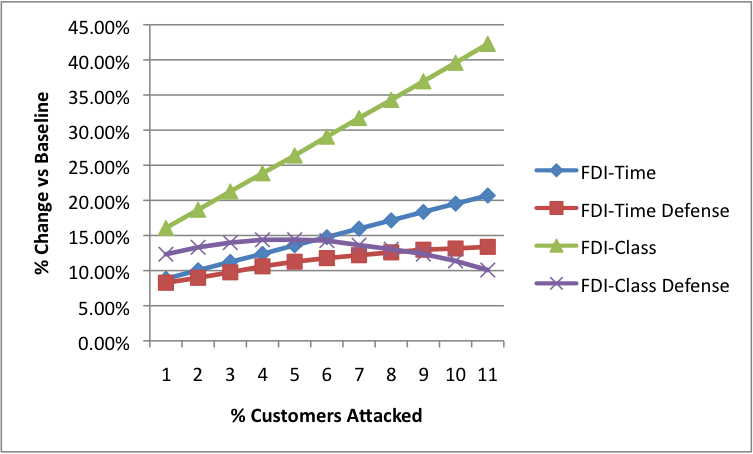
\includegraphics[width=.5\textwidth]{unequal-attacks.png}
\caption{Attack strategies with different numbers of customers in each class}
\label{unequal-attack}
\end{figure}

Figure \ref{unequal-attack} shows the results for the second scenario with 6,000 Bakeries and Batteries, and 3,000 Buckets.  The overall results here are roughly the same as for scenario one.  The item of interest is that the defense for false data injection - class becomes more and more effective as more customers are attacked.  This attack converts Buckets into Bakeries.  The efficacy of the defense highlights the critical flexibility that Buckets provide for the utility.

